\section{RELATED WORK AND BACKGROUND}

\subsection{Pattern prediction over event streams}


\subsubsection*{Related work:\\}
The task of forecasting over time-evolving streams of data can be formulated in various different ways and with varying assumptions.
One of the most usual ways to formalize this task is to assume that the stream is a time-series of numerical values and the goal is to forecast at each time point $n$ the values at some future points $n+1$, $n+2$, etc. (or even the output of some function of future values). 
This is the task of time-series forecasting \cite{montgomery_introduction_2015}.
Another way to formalize this task is to view streams as sequences of events,
i.e., tuples with multiple, possibly categorical, attributes, like \textit{event type}, \textit{timestamp}, etc. 
In this work that we present here, 
we focus on this latter definition of forecasting (event forecasting).  

A substantial body of work on event forecasting comes from the field of temporal pattern mining where events are defined as 2-tuples of the form $(\mathit{EventType},\mathit{Timestamp})$.
The ultimate goal is to extract patterns of events in the form either of association rules \cite{agrawal_mining_1993} or frequent episode rules \cite{mannila_discovery_1997}. 
These methods have been extended in order to be able to learn not only rules for detecting event patterns but also rules for predicting events.
For example, in \cite{vilalta_predicting_2002}, a variant of association rule mining is where the goal is to extract sets of event types that frequently lead to a rare, target event within a temporal window. 
In \cite{laxman_stream_2008}, a probabilistic model is presented
in order to calculate the probability of the immediately next event in the stream. 
This is achieved by using standard frequent episode discovery algorithms and combining them with Hidden Markov Models and mixture models.
The framework of episode rules is employed in \cite{fahed_efficient_2014} as well.
The output of the proposed algorithms is a set predictive rules whose antecedent is minimal (in number of events) and temporally distant from the consequent.
In \cite{zhou_pattern_2015} a set of algorithms is proposed that target batch, online mining of sequential patterns, without maintaining exact frequency counts.
As the stream is consumed, the learnt patterns can be used to test whether a prefix matches the last events seen in the stream, 
indicating a possibility of occurrence for events that belong to the suffix of the rule.

Event forecasting has also attracted some attention from the filed of Complex Event Processing (see \cite{Cugola:2012:PFI:2187671.2187677} for a review).
One such early approach is presented in \cite{muthusamy_predictive_2010}.
Complex event patterns are converted to automata and subsequently
Markov chains are used in order to estimate when a pattern is expected to be fully matched.
A similar approach is presented in \cite{alevizos2017event},
where again automata and Markov chains are employed in order to provide (future) time intervals during which a match is expected with a probability above a confidence threshold. 

\subsubsection*{Event forecasting with pattern Markov Chains:\\}

For our work presented in this paper,
we use the approach described in \cite{alevizos2017event}.
For the sake of self-containment,
we briefly describe this approach in what follows.

The problem at hand may be stated as follows: given a stream of low-level events and a pattern defining relations between low-level events, 
in the form of a regular expression (i.e., using operators for \textit{sequence}, \textit{disjunction} and \textit{iteration}),
the goal is to estimate at each new event arrival the number of future events
that we will need to wait for until the expression is satisfied (and therefore a match be detected).

As a first step, event patterns are converted to deterministic finite automata (DFA) through standard conversion algorithms.
As an example, see Figure \ref{fig:dfatcc} for the DFA of the simple sequential pattern $R=a\cdot c\cdot c$ and an alphabet $\Sigma=\{a,b,c\}$
(note that the DFA has no dead states since we need to handle streams and not strings).
The next step is to derive a Markov chain that will be able to provide a probabilistic description of the DFA's run-time behavior.
Towards this goal, we use Pattern Markov Chains, as  proposed in \cite{nuel_pattern_2008}.
Under the assumption that the input events are independent and identically distributed (i.i.d.), it can be shown that there is a direct mapping of the states of the DFA to states of a Markov chain and the transitions of the DFA to transitions of the Markov chain.
The transition probabilities of the Markov chain are the occurrence probabilities of the various event types.
On the other hand, if the occurrence probabilities of the events are dependent on some of the previous events seen in the stream 
(i.e., the stream is generated by an $m^{th}$ order Markov process),
we might need to perform a more complex transformation 
(see \cite{nuel_pattern_2008} for details)
in order to obtain a ``proper'' Markov chain.
The transition probabilities are then conditional probabilities on the event types.
In any case,
we call such a derived Markov chain a Pattern Markov Chain (PMC) of order m
and denote by \pmcmr , where $R$ is the initial pattern and $m$ the assumed order.
As an example, see Figure \ref{fig:mctcc1}, which depicts the PMC of order 1 for the DFA of Figure \ref{fig:dfatcc}.
%\begin{comment}
\begin{figure}[!ht]
\begin{centering}
\subfloat[\dfasr]{
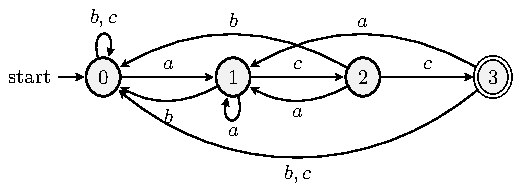
\includegraphics[height=0.105\textheight,width=\linewidth]{./figures/forecasting/dfasr.pdf}
\label{fig:dfatcc}
}
\hfill
\subfloat[\pmconer]{
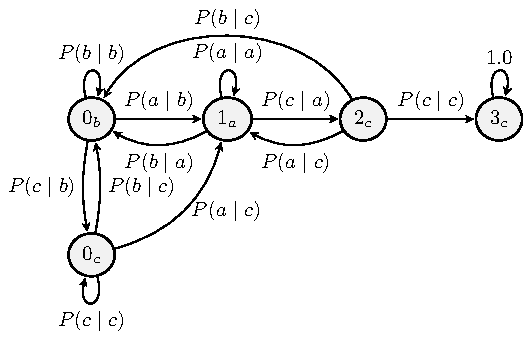
\includegraphics[width=0.35\textwidth]{./figures/forecasting/pmcr1.pdf}
\label{fig:mctcc1}
}
%\hfill
\caption{DFA and PMC for $R=a\cdot c\cdot c$,  $\Sigma=\{a,b,c\}$ and $m=1$.}
\label{fig:dfa_mc_example}
\end{centering}
\end{figure}
%\end{comment}


After constructing a PMC, we can use it in order to calculate the so-called \textit{waiting-time} distributions.
Given a specific state of the PMC, a \textit{waiting-time} distribution gives us the probability of reaching a set of absorbing states in $k$ transition from now (absorbing states are states with self-loops and probability equal to $1.0$).
By mapping the final states of the initial DFA to absorbing states of the PMC
(see again Figure \ref{fig:dfa_mc_example}),
we can therefore calculate the probability of reaching a final state,
or, in other words, of detecting a full match of the original regular expression in $k$ events from now.

In order to estimate the final forecasts, another step is required,
since our aim is not to provide a single future point with the highest probability but an interval. 
Forecasts are given in the form of intervals, like $I=(\mathit{start},\mathit{end})$. 
The meaning of such an interval is that the DFA is expected to reach a final state sometime in the future between $\mathit{start}$ and $\mathit{end}$ with probability at least some constant threshold $\theta_{fc}$ (provided by the user). 
These intervals are estimated by a sinlge-pass algorithm that scans a waiting-time distribution and finds the smallest (in terms of length) interval that exceeds this threshold. 
An example is shown in Figure \ref{fig:wtdfas},
where the DFA in Figure \ref{fig:dfa1} is in state $1$,
the \textit{waiting-time} distributions for all of its non-final states are shown in Figure \ref{fig:wt1}
and the distribution, along with the forecast interval, for state $1$ are shown in green.
\begin{figure}[!ht]
\begin{centering}
\subfloat[DFA, state 1.]{ 
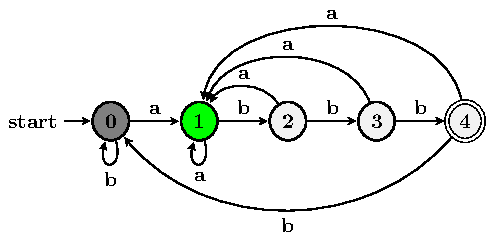
\includegraphics[width=0.15\textwidth,height=0.12\textheight]{./figures/forecasting/dfa1.pdf}
\label{fig:dfa1}
}
\subfloat[Waiting-time distribution, state 1.]{ 
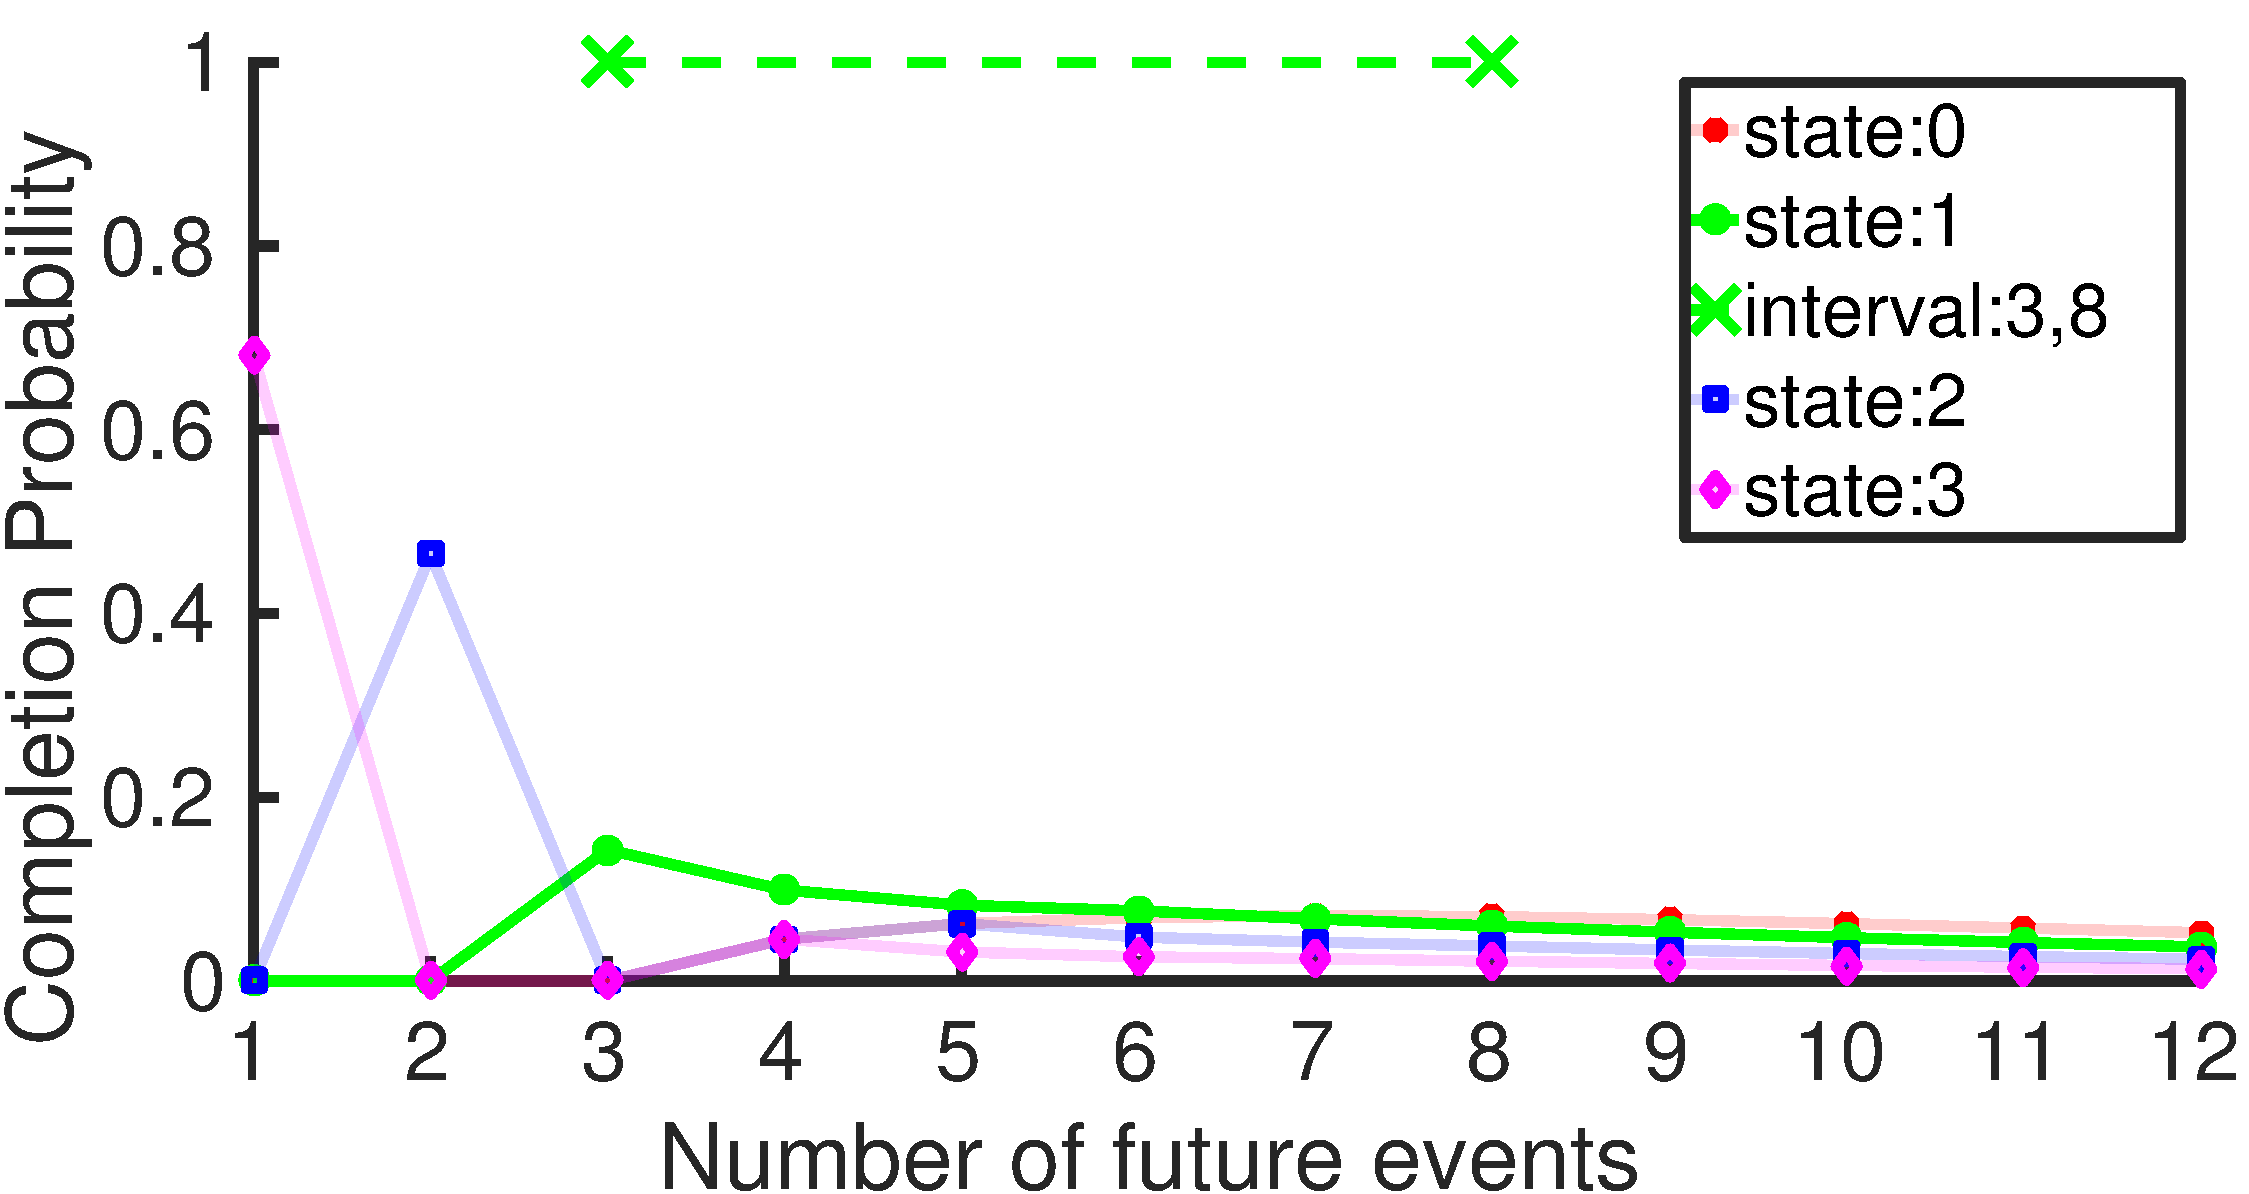
\includegraphics[width=0.3\textwidth,height=0.16\textheight]{./figures/forecasting/wt1.pdf}
\label{fig:wt1}
}
\caption{Example of how forecasts are produced. 
$R=a\cdot b\cdot b\cdot b$, $\Sigma=\{a,b\}$, $m=1$, $\theta_{\mathit{fc}}=0.5$.}
\label{fig:wtdfas}
\end{centering}
\end{figure}

The above described method assumes that we know the (possibly conditional) occurrence probabilities of the various event types appearing in a stream
(as would be the case with synthetically generated streams).
However, this is not always the case in real-world situations.
Therefore, it is crucial for a system implementing this method to have the capability to learn the values of the PMC's transition matrix.
One way to do this is to use some part of the stream to obtain the maximum-likelihood estimators for the transition probabilities. 
If $\boldsymbol{\Pi}$ is the transition matrix of a Markov chain with a set of states $Q$, 
$\pi_{i,j}$ the transition probability from state $i$ to state $j$,
$n_{i,j}$ the number of transitions from state $i$ to state $j$,
then the maximum likelihood estimator for $\pi_{i,j}$ is given by:
\begin{equation*}
\label{eq:pi_estim}
\hat{\pi}_{i,j}=\frac{n_{i,j}}{\sum_{k \in Q} n_{i,k}}=\frac{n_{i,j}}{n_{i}}
\end{equation*}
Executing this learning step on a single node might require a substantial amount of time until we arrive at a sufficiently good model.
In what follows, we present a distributed method for learning the transition matrix.
